\documentclass[tikz]{standalone}
\usepackage{ifthen}
\usepackage{amsmath}
\usepackage{tikz}
\usetikzlibrary{positioning, graphs, calc}
\usetikzlibrary{graphs.standard}
\begin{document}
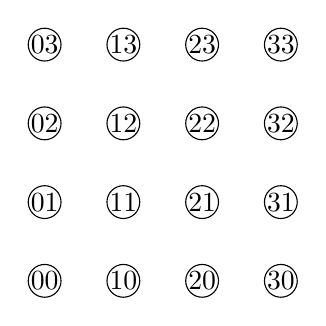
\begin{tikzpicture}
		[every node/.style={draw,circle,inner sep = 0mm, minimum size = 2mm}]
		\foreach \i in {0, ..., 3}
			\foreach \j in {0, ..., 3}{
				\draw (\i, \j) node {\i\j};
			}
		\foreach \i in {0, ..., 3}{
			\foreach \j in {0, ..., 3}{
				\foreach \k in {0, ..., 3}{
					\foreach \l in {0, ..., 3}{
						\pgfmathparse{\i - \k}\let\difx\pgfmathresult
						\pgfmathparse{\j - \l}\let\dify\pgfmathresult
						%\ifthenelse{\(\not\(\difx=0\)\)\AND\(\not\(\dify=0\)\)}{
							%\ifthenelse{\(\difx=2\)\OR\(\dify=2\)}{
								%\draw (\i, \j) -- (\k, \l);
							%}{}
						%}
					}
				}
			}
		}
\end{tikzpicture}
\end{document}